\documentclass[conference]{IEEEtran}

\usepackage{amsmath}
\usepackage{booktabs}
\usepackage{graphicx}
\usepackage{microtype}
\usepackage{xcolor}
\usepackage{url}

\graphicspath{{figures/}}
\raggedbottom

\title{GNN--BERT for Understanding Context from Music}

\author{\IEEEauthorblockN{Moin Mostakim}
\IEEEauthorblockA{Department of Computer Science and Engineering\\
Course: Neural Networks (CSE425 / EEE474 / CSE715)\\
Email: \textit{[add institutional email]}}}

\begin{document}
\maketitle

\begin{abstract}
Music context is distributed across acoustic structure and language. This
paper presents a three-stage study of text-only, audio-graph, and graph--text
models for music understanding. A DistilBERT baseline is evaluated on a
MusicCaps caption-to-tag proxy task. FMA-small tracks are represented as
graphs of five-second audio segments for genre classification with GraphSAGE,
and compared with a mel-spectrogram CNN. A graph--text model predicts a fixed
multi-label genre/tag
vocabulary from FMA metadata text and audio graphs, comparing BERT-only,
GNN-only, early-concatenation, and cross-attention fusion. On the reported
test runs, the CNN obtains macro-F1 $0.4544$ versus $0.4323$ for
GraphSAGE. In the multimodal ablation, graph-only obtains the best macro-F1
($0.0427$) and
mean PR-AUC ($0.1340$), while cross-attention obtains the best micro-F1
($0.3546$). The results show that graph structure supplies useful signal for
the selected FMA labels, but also expose substantial generalization
difficulties for the multi-label fusion setting.
\end{abstract}

\begin{IEEEkeywords}
music understanding, GraphSAGE, BERT, multimodal learning, audio graphs,
multi-label classification
\end{IEEEkeywords}

\section{Introduction}
Music context includes timbre, rhythm, harmony, genre, mood, and natural
language descriptions. Audio-only sequence models capture local patterns but
do not explicitly represent relations between repeated or similar segments.
Conversely, a language encoder captures contextual semantics but cannot
directly observe acoustic structure. We study whether a graph representation
of audio segments and a BERT representation of metadata text can provide
complementary information.

We consider three complementary settings. A DistilBERT baseline measures
text-only performance on a caption-to-tag proxy task. A GraphSAGE model
performs single-label genre classification from audio-segment graphs and is
compared with a mel-spectrogram CNN. Finally, a graph--text model performs
multi-label genre/tag prediction through a four-condition ablation. Results
from synthetic data are used only to validate the implementation and are not
included as experimental evidence.

\section{Related Work}
The language branch is based on the contextual representation strategy of
BERT \cite{devlin2019bert}; the implementation uses the smaller
DistilBERT configuration for the text-only baseline
\cite{sanh2019distilbert}. GraphSAGE learns node representations by sampling
and aggregating neighborhood information \cite{hamilton2017inductive}.
The audio features use standard short-time spectral analysis and
mel-spectrogram conventions \cite{mcfee2015librosa}. FMA provides the
audio and metadata basis for genre classification and fusion
\cite{defferrard2017fma}, while MusicCaps supplies natural-language
descriptions for the caption-to-tag proxy experiment
\cite{agostinelli2023musiclm}.

\section{Data and Prediction Targets}
\subsection{Datasets and targets}
The text-only experiment uses real MusicCaps captions and a proxy tag target
generated from the captions. This target is not a human-annotated
MusicCaps tagging benchmark, so its score is reported separately from the
FMA experiments. The audio and multimodal experiments use FMA-small. Genre
classification is single-label over eight top-level genres:
Electronic, Experimental, Folk, Hip-Hop, Instrumental, International, Pop,
and Rock.

The multimodal experiment uses the complete FMA metadata source and constructs a fixed
multi-label vocabulary. Normalized genres are included first and frequent
normalized tags fill the remaining positions up to the configured maximum
of 100 labels. The target is multi-hot: a track is positive for its normalized
top genre and any selected normalized tags. The exact vocabulary is persisted
by the preparation pipeline and reused across all four ablation conditions.

\subsection{Splits and leakage control}
All partitions are artist-disjoint: every track from an artist
from one artist belong to exactly one of train, validation, or test. The
fusion manifest is an inner join on \texttt{track\_id} between the graph
manifest and prepared text metadata, so failed graph construction and rows
without usable text are excluded consistently. Feature scaling is fitted on
training segments and shared across splits. These choices prevent direct
artist leakage and prevent test statistics from influencing graph features.

\section{Method}
\subsection{Audio segmentation and graph construction}
Audio is loaded as mono at 22{,}050 Hz and partitioned into five-second
segments. Each segment node contains MFCC means and standard deviations,
first- and second-order MFCC deltas, chroma statistics, spectral contrast,
tonnetz, spectral centroid, bandwidth, rolloff, zero-crossing rate, RMS
energy, and spectral-flatness statistics. The resulting feature dimension is
182. Temporal-adjacency edges connect consecutive segments. Additional
undirected similarity edges are added when the cosine similarity of the
complete audio feature vectors is at least $0.75$.

The graph encoder projects node features to a 256-dimensional hidden
space, applies three residual GraphSAGE layers with normalization and
dropout, and concatenates mean, maximum, and standard-deviation global
readouts. A linear head maps the graph representation to the target labels.
The corresponding convolutional baseline applies a compact CNN to a
128-bin log-mel spectrogram.

\subsection{Text and fusion models}
The text-only baseline uses a DistilBERT encoder with a linear multi-label
head. The multimodal model passes only non-target FMA metadata text to BERT:
album information, album
title/type, artist biography/location/members, composer, track information,
and track title. Genre/tag fields, identifiers, dates, URLs, and split
metadata are excluded from the text input.

Let $g$ denote the graph readout and $H$ the BERT token sequence. The
cross-attention condition uses a graph-derived query:
\begin{equation}
 A = \operatorname{softmax}\left(\frac{(gW_Q)(HW_K)^\top}{\sqrt{d}}\right),
 \qquad
 z = [g;\, AHW_V].
\end{equation}
The early-concatenation condition replaces the attended text vector with the
BERT pooled output. The text-only and graph-only conditions remove the other
branch. All multimodal conditions use binary cross-entropy with logits, and
predictions are thresholded at $0.5$ for F1.

\subsection{Evaluation}
Macro-F1, micro-F1, and mean average precision (reported by the
implementation as mean PR-AUC) are reported for multi-label prediction.
Accuracy and test loss are additionally reported for genre classification.
Checkpoints are selected on the validation split, and all reported scores
are computed on held-out test data.

\section{Experimental Setup and Reproducibility}
\subsection{Data preparation and validation}
The implementation was validated first on controlled synthetic graphs with
six labels, random node features, deterministic splits, and serialized graph
manifests. This preliminary check verified tensor shapes, checkpoint
serialization, evaluation, and qualitative-output generation; synthetic
scores are not used in the analysis below.

The reported experiments use a stable 80/10/10 split for the MusicCaps
caption proxy and artist-disjoint train/validation/test partitions for FMA.
The audio pipeline constructs metadata, segment graphs, and cached
mel-spectrograms separately. Feature extraction was expanded from MFCC-only
representations to include harmonic, spectral, rhythm, and energy
statistics; normalization is fitted on training segments before similarity
edges are constructed. The multimodal pipeline scans and normalizes genres
and tags, selects a deterministic vocabulary, creates non-target descriptive
text, and joins graph and text records by track identifier. These procedures
provide a common data contract for the ablation models.
The resulting preparation and validation stages are summarized in
Table~\ref{tab:milestones}.

\begin{table*}[t]
\caption{Data preparation and validation procedures.}
\label{tab:milestones}
\centering
\small
\begin{tabular}{p{0.17\textwidth}p{0.27\textwidth}p{0.46\textwidth}}
\toprule
Procedure & Purpose & Evidence\\
\midrule
Preliminary validation & Can graph/text training and evaluation run end to end? &
\texttt{src/make\_synthetic\_data.py}, synthetic manifest, checkpoints, and case-study generation\\
Text baseline & Can contextual text encode the proxy labels? &
MusicCaps preparation, DistilBERT checkpoint, metric history, predictions, F1 curve\\
Data and layout & Which datasets and directory contracts are valid? &
FMA and MusicCaps data definitions, processing conventions, and experiment paths\\
Audio preprocessing & Can real audio become leakage-controlled graphs and cached mels? &
FMA metadata, audio features, scaling, graph manifest, split files, failure report, mel cache\\
Audio modeling & Does graph structure beat a standard spectrogram baseline? &
GraphSAGE/CNN checkpoints, learning curves, confusion matrices, predictions, comparison JSON\\
Multimodal preparation & Can labels and text be built without target leakage? &
Scan/select/prepare commands, fixed vocabulary, prepared text, inner-join manifest, validators\\
Fusion ablation & Which modality and fusion mechanism contributes? &
Four checkpoints, histories, predictions, PR curves, t-SNE plots, case studies, comparison analysis\\
\bottomrule
\end{tabular}
\end{table*}

\subsection{Configuration and reproducibility}
Unless overridden by a task command, experiments use seed 42, batch size 8,
learning rate $3\times10^{-4}$, weight decay $10^{-4}$, dropout 0.2, three
GraphSAGE layers, 256-dimensional graph and text projections, gradient
clipping at 1.0, a factor-0.5 learning-rate scheduler, and early stopping
with patience 12. The text baseline uses DistilBERT, maximum sequence length 128,
batch size 8, learning rate $2\times10^{-5}$, and the documented real run.
The graph and multimodal experiments use the same seed/configuration
contract; multimodal runs are capped at 20 epochs and select the best
validation Macro-F1 checkpoint. The primary fusion run uses positive
weighting, and every ablation uses the same fixed label order. The
consolidated settings are listed in
Table~\ref{tab:hyperparameters}.

\begin{table}[!ht]
\caption{Core experimental hyperparameters.}
\label{tab:hyperparameters}
\centering
\begin{tabular}{ll}
\toprule
Parameter & Value\\
\midrule
Seed & 42\\
Audio sample rate / segment & 22,050 Hz / 5 s\\
Mel bins / similarity threshold & 128 / 0.75\\
Graph layers / hidden size & 3 / 256\\
Text model / max length & DistilBERT / 128\\
Dropout / batch size & 0.2 / 8\\
Learning rate / weight decay & $3\times10^{-4}$ / $10^{-4}$\\
Scheduler / early stopping & factor 0.5 / patience 12\\
Gradient clipping & 1.0\\
Multimodal loss & BCEWithLogitsLoss\\
\bottomrule
\end{tabular}
\end{table}

\section{Experiments and Results}
\subsection{Caption-to-tag proxy classification}
The DistilBERT test evaluation reports macro-F1 $0.9976$, micro-F1
$0.9991$, and PR-AUC $1.0000$. Because the experiment uses caption-derived
proxy labels, these values should be interpreted as a verification of the
text pipeline and not as evidence of general MusicCaps tag understanding.
The training trajectory in Fig.~\ref{fig:task1-curve} reaches a similarly
high validation score quickly, consistent with the proxy nature of the target
rather than difficult semantic generalization. The held-out values are
reported in Table~\ref{tab:task1}.

\begin{table}[!ht]
\caption{DistilBERT test performance on the MusicCaps caption-to-tag proxy.}
\label{tab:task1}
\centering
\begin{tabular}{lccc}
\toprule
Model & Macro-F1 & Micro-F1 & PR-AUC\\
\midrule
DistilBERT & 0.9976 & 0.9991 & 1.0000\\
\bottomrule
\end{tabular}
\end{table}

\begin{figure}[!ht]
\centering
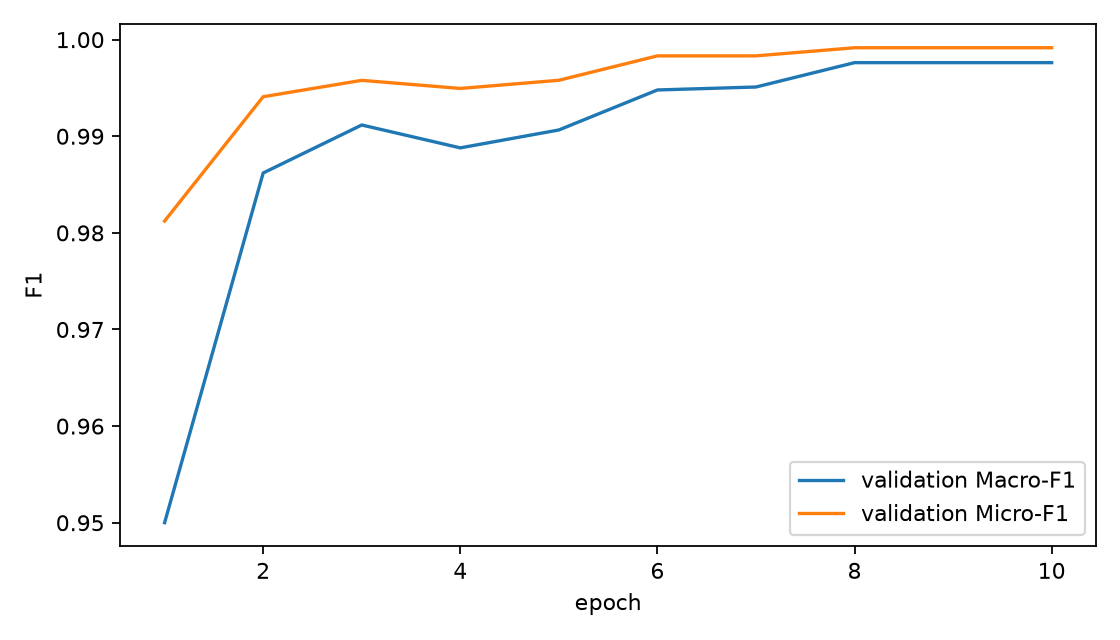
\includegraphics[width=\columnwidth]{task1_distilbert_f1_curve.png}
\caption{DistilBERT training and validation F1 curves on the
MusicCaps caption-to-tag proxy task.}
\label{fig:task1-curve}
\end{figure}

\subsection{Audio-graph genre classification}
Table~\ref{tab:task2} compares GraphSAGE with the mel-spectrogram CNN.
The CNN leads GraphSAGE by 0.0222 macro-F1 and 0.0350 PR-AUC, while both
models achieve their best per-class F1 on Hip-Hop. GraphSAGE is stronger on
International, whereas the CNN is stronger on Experimental, Folk, Hip-Hop,
Instrumental, Pop, and Rock.

\begin{table}[!ht]
\caption{FMA-small genre classification test results.}
\label{tab:task2}
\centering
\begin{tabular}{lccccc}
\toprule
Model & Acc. & Macro-F1 & Micro-F1 & PR-AUC & Loss\\
\midrule
Mel-CNN & 0.4650 & 0.4544 & 0.4650 & 0.4939 & 1.4877\\
GraphSAGE & 0.4300 & 0.4323 & 0.4300 & 0.4534 & 1.7490\\
\bottomrule
\end{tabular}
\end{table}

\begin{table}[!ht]
\caption{Per-genre test F1 on FMA-small. Bold values indicate the stronger model
for each genre; the final column is CNN minus GraphSAGE.}
\label{tab:task2-perclass}
\centering
\scriptsize
\begin{tabular}{lccc}
\toprule
Genre & Mel-CNN & GraphSAGE & $\Delta$\\
\midrule
Electronic & 0.5510 & \textbf{0.5771} & -0.0261\\
Experimental & \textbf{0.3814} & 0.2880 & +0.0934\\
Folk & \textbf{0.2647} & 0.2513 & +0.0134\\
Hip-Hop & \textbf{0.7444} & 0.6900 & +0.0544\\
Instrumental & \textbf{0.4330} & 0.3209 & +0.1121\\
International & 0.3467 & \textbf{0.4852} & -0.1385\\
Pop & 0.3333 & \textbf{0.3491} & -0.0157\\
Rock & \textbf{0.5809} & 0.4967 & +0.0842\\
\midrule
Macro-F1 & \textbf{0.4544} & 0.4323 & +0.0222\\
\bottomrule
\end{tabular}
\end{table}

\noindent
The per-genre breakdown in Table~\ref{tab:task2-perclass} is more informative
than accuracy alone: GraphSAGE
improves Electronic, International, and Pop, while the CNN has larger gains
on Experimental, Instrumental, and Rock. Both models are strongest on
Hip-Hop, suggesting that class separability and class frequency are not
uniform across the eight genres. The learning curves in
Fig.~\ref{fig:task2-curves} and Fig.~\ref{fig:task2-graph-curves} show the
optimization behavior behind the final comparison, while the confusion
matrices in Fig.~\ref{fig:task2-confusion}
and Fig.~\ref{fig:task2-graph-confusion} make class-specific errors visible.
The corresponding GraphSAGE learning trajectory is shown in
Fig.~\ref{fig:task2-graph-curves}.

\begin{figure}[!ht]
\centering
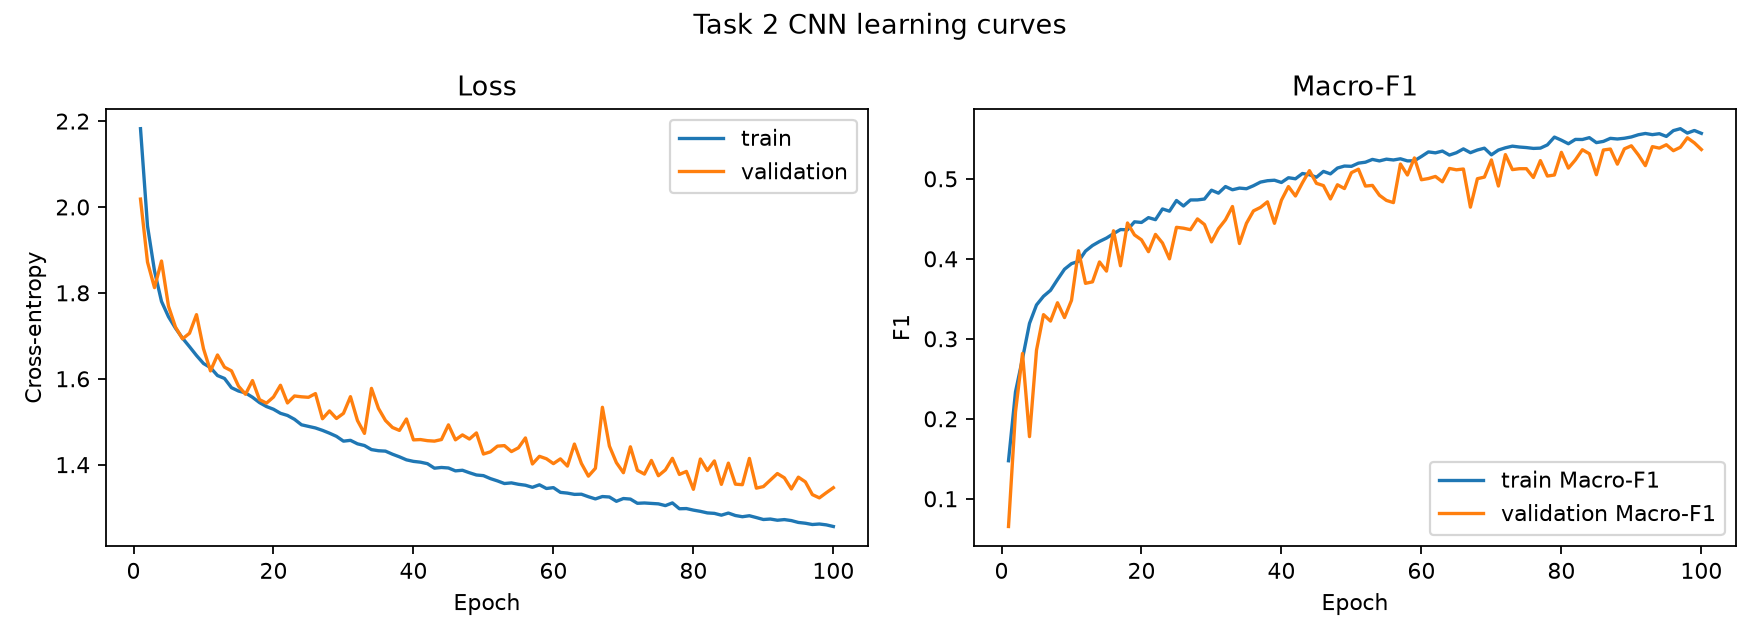
\includegraphics[width=\columnwidth]{task2_cnn_learning_curves.png}
\caption{Mel-spectrogram CNN learning curves.}
\label{fig:task2-curves}
\end{figure}

\begin{figure}[!ht]
\centering
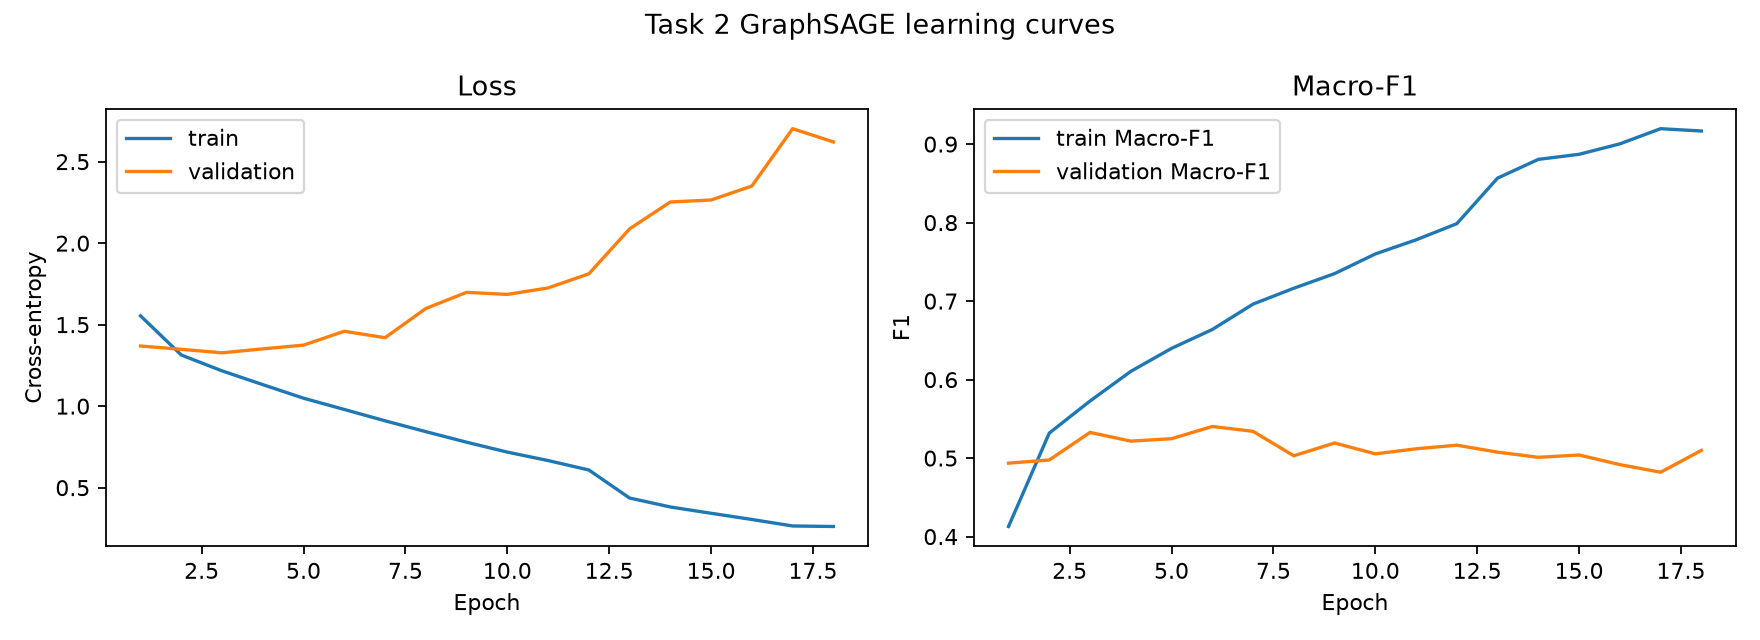
\includegraphics[width=\columnwidth]{task2_graphsage_learning_curves.png}
\caption{GraphSAGE learning curves.}
\label{fig:task2-graph-curves}
\end{figure}

\begin{figure}[!ht]
\centering
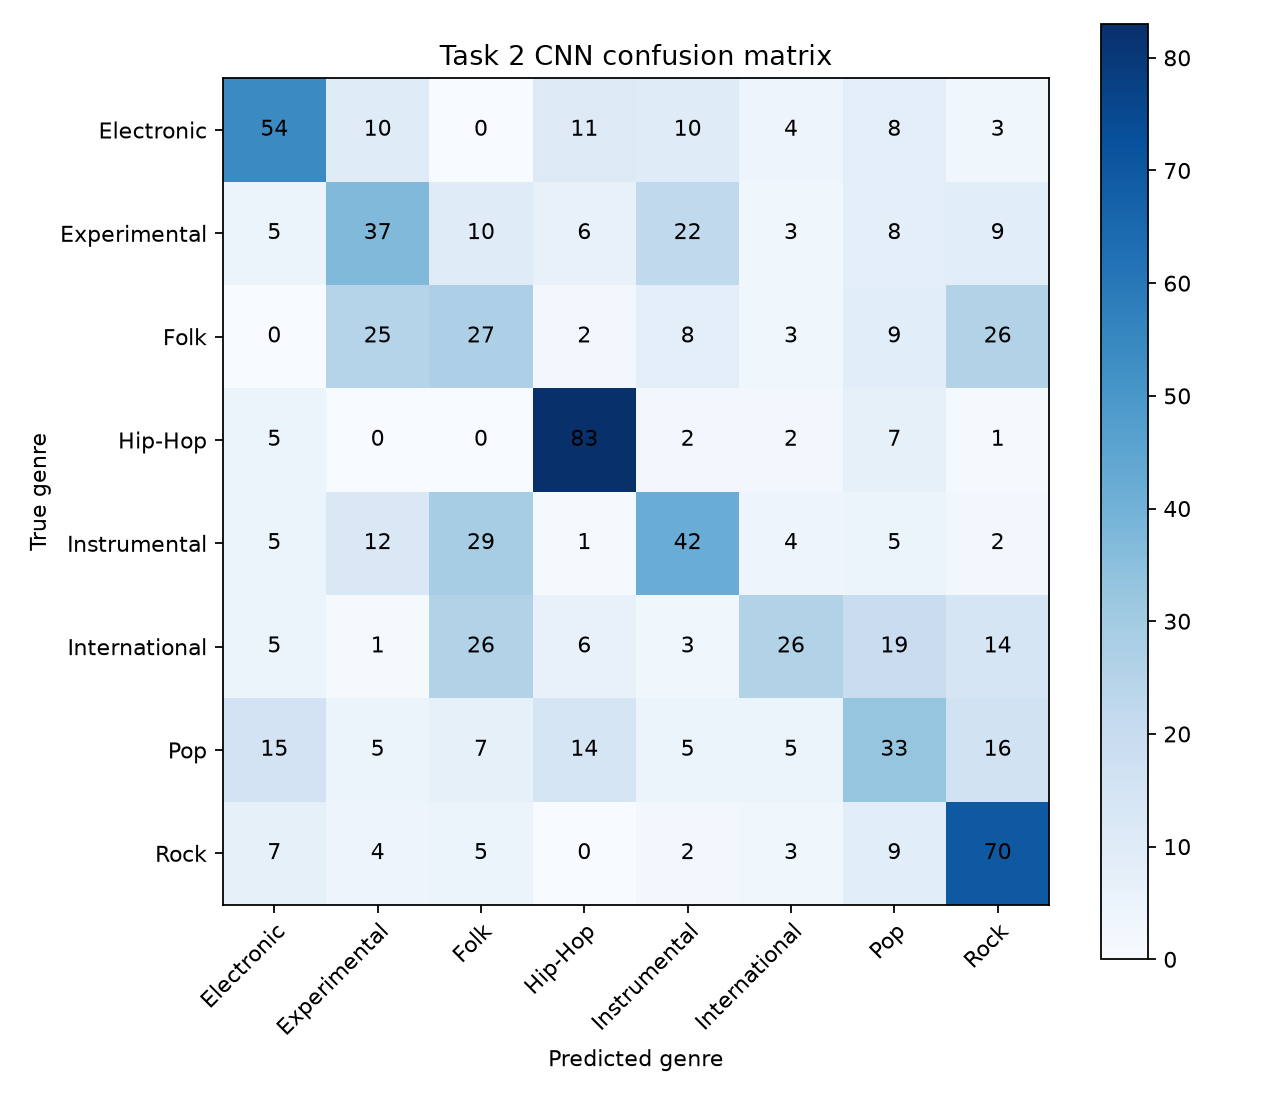
\includegraphics[width=\columnwidth]{task2_cnn_confusion_matrix.png}
\caption{Mel-spectrogram CNN test confusion matrix.}
\label{fig:task2-confusion}
\end{figure}

\begin{figure}[!ht]
\centering
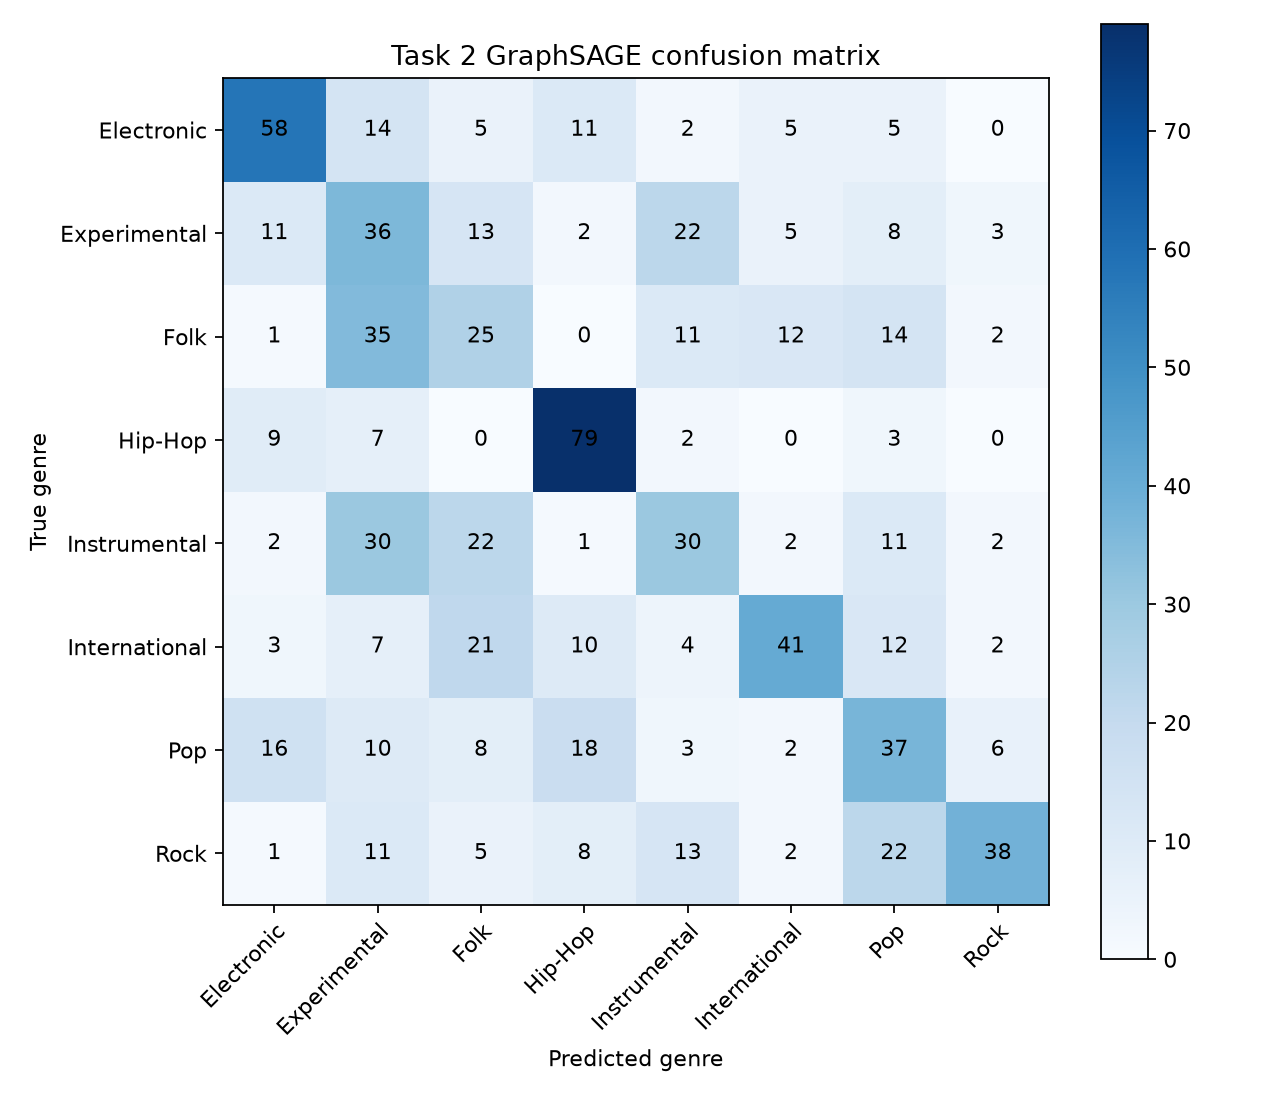
\includegraphics[width=\columnwidth]{task2_graphsage_confusion_matrix.png}
\caption{GraphSAGE test confusion matrix.}
\label{fig:task2-graph-confusion}
\end{figure}

\subsection{Multimodal fusion ablation}
The four-condition results are shown in Table~\ref{tab:task3}. The graph-only
achieves the highest macro-F1 and PR-AUC. Cross-attention achieves the
highest micro-F1, narrowly exceeding early concatenation. Both fusion
conditions substantially improve on BERT-only micro-F1 and PR-AUC, but their
macro-F1 remains low, indicating that performance is concentrated in a
subset of labels. The gap between training and test metrics in the exported
histories also indicates overfitting.

\begin{table}[!ht]
\caption{FMA multi-label ablation test results.}
\label{tab:task3}
\centering
\begin{tabular}{lccc}
\toprule
Condition & Macro-F1 & Micro-F1 & PR-AUC\\
\midrule
BERT-only & 0.0111 & 0.2030 & 0.0366\\
GNN-only & \textbf{0.0427} & 0.3353 & \textbf{0.1340}\\
Early concat. & 0.0403 & 0.3542 & 0.1255\\
Cross-attention & 0.0393 & \textbf{0.3546} & 0.1308\\
\bottomrule
\end{tabular}
\end{table}

\begin{table}[!ht]
\caption{Improvement over the text-only test baseline. Positive
values are improvements for F1 and PR-AUC; for loss, negative values would
be improvements.}
\label{tab:task3-deltas}
\centering
\begin{tabular}{lrrrr}
\toprule
Condition & $\Delta$ Macro-F1 & $\Delta$ Micro-F1 & $\Delta$ PR-AUC & $\Delta$ Loss\\
\midrule
BERT-only & 0.0000 & 0.0000 & 0.0000 & 0.0000\\
GNN-only & +0.0315 & +0.1323 & +0.0974 & +1.3756\\
Early concat. & +0.0292 & +0.1512 & +0.0889 & +0.4578\\
Cross-attention & +0.0281 & \textbf{+0.1516} & +0.0942 & +0.6663\\
\bottomrule
\end{tabular}
\end{table}

\noindent
The delta table is useful because the absolute scores alone hide
the practical effect of adding audio. Cross-attention gives the largest
micro-F1 improvement, while GNN-only gives the largest macro-F1 and PR-AUC
improvements. None of the audio-containing conditions minimizes BCE test
loss, so the result is not a uniformly dominant fusion model. These
baseline-relative changes are reported in Table~\ref{tab:task3-deltas}. The visual
comparison in Fig.~\ref{fig:task3-comparison} reinforces this
metric-dependent ranking.

\begin{figure}[!ht]
\centering
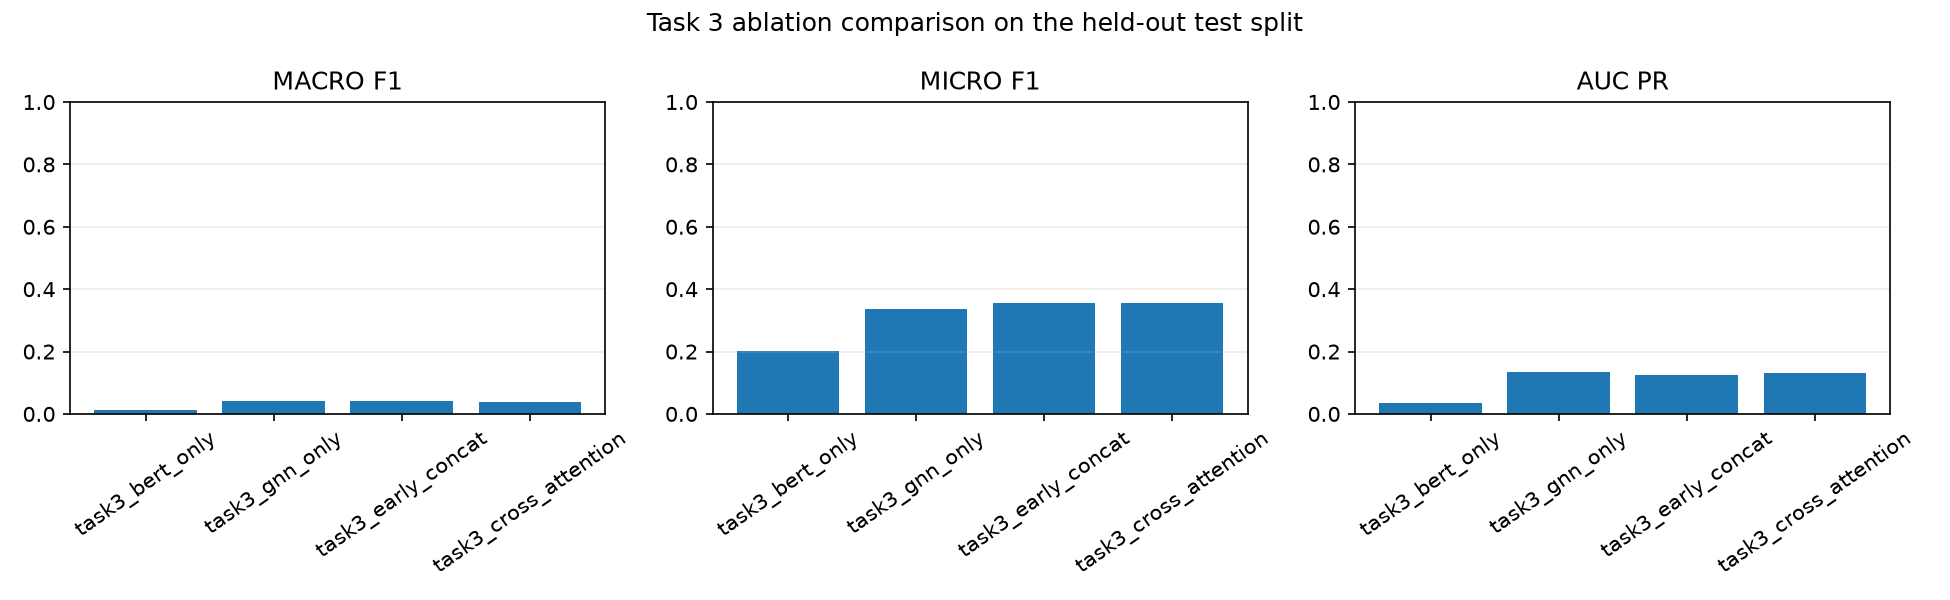
\includegraphics[width=\columnwidth]{task3_ablation_comparison.png}
\caption{Multimodal ablation comparison across Macro-F1, Micro-F1, and PR-AUC.}
\label{fig:task3-comparison}
\end{figure}

\subsection{Training dynamics and comparative analysis}
The training histories provide evidence beyond the final test row. The
text baseline reaches its best validation Macro-F1 at epoch 4 in the stored
history. The graph-only and fusion conditions reach their best stored
validation Macro-F1 at epoch 5, while BERT-only reaches its best at epoch 2.
The large train/test gaps, especially for GNN-only and fusion, indicate
overfitting and label imbalance rather than a lack of optimization alone.

Relative to BERT-only, the post-ablation analysis reports the following
cross-attention changes: Macro-F1 +0.0281, micro-F1 +0.1516, PR-AUC
+0.0942, and test loss +0.6663. Thus adding audio improves micro-level
decisions and ranking quality, but the improvement is not uniform over
labels. The ranking is metric-dependent: GNN-only is best for Macro-F1 and
PR-AUC, cross-attention is best for micro-F1, and BERT-only has the lowest
test loss.
For the selected primary fusion run, Fig.~\ref{fig:task3-crossattn-curves}
shows the train/validation history and Fig.~\ref{fig:task3-crossattn-pr}
shows per-label precision--recall behavior. These figures support the
overfitting and imbalance interpretation; Table~\ref{tab:task3} remains the
primary cross-model evidence. The corresponding checkpoint epochs and test
Macro-F1 values are summarized in Table~\ref{tab:epochs}.

\begin{table}[!ht]
\caption{Best validation epochs and corresponding test Macro-F1.}
\label{tab:epochs}
\centering
\begin{tabular}{lcc}
\toprule
Run & Best epoch & Test Macro-F1\\
\midrule
DistilBERT proxy & 4 & 0.0409\\
Text-only & 2 & 0.0111\\
Graph-only & 5 & 0.0427\\
Early concat. & 5 & 0.0403\\
Cross-attention & 5 & 0.0393\\
\bottomrule
\end{tabular}
\end{table}

\begin{figure}[!ht]
\centering
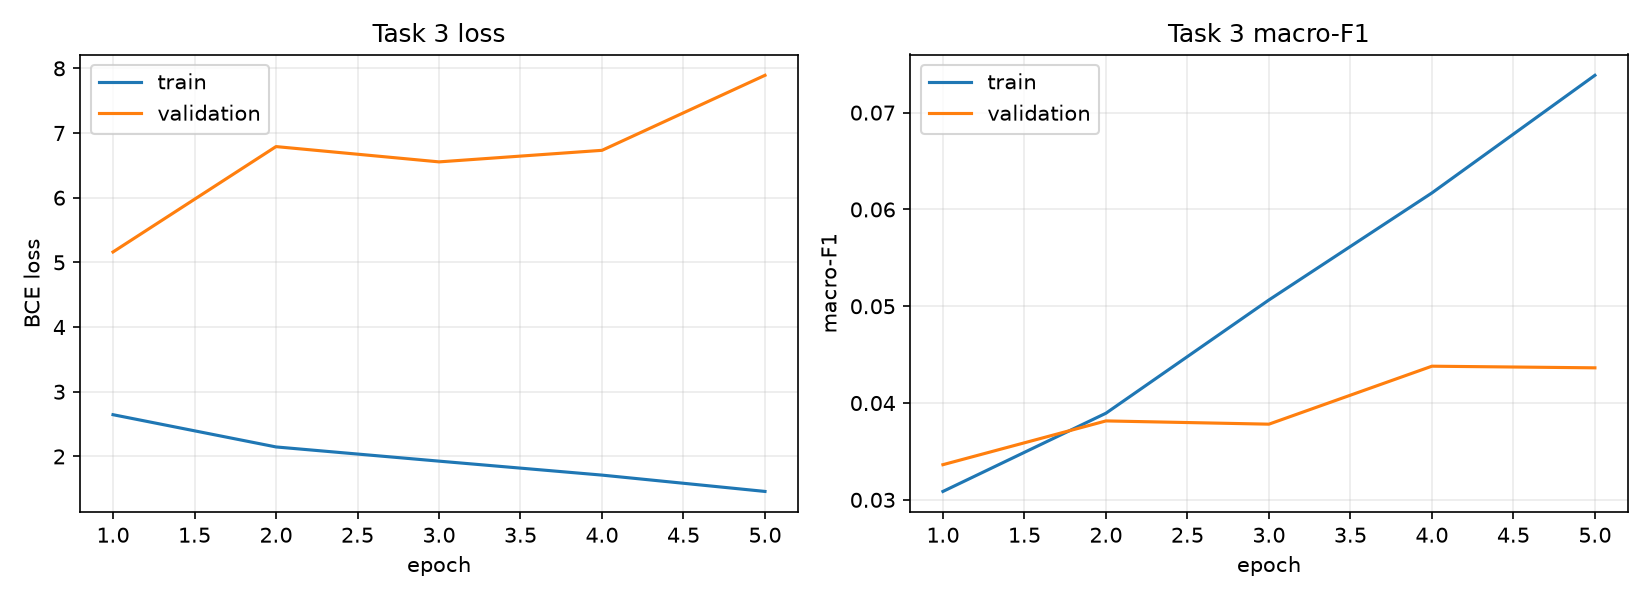
\includegraphics[width=\columnwidth]{task3_cross_attention_learning_curves.png}
\caption{Cross-attention training and validation history. The widening
training--validation gap motivates the overfitting interpretation.}
\label{fig:task3-crossattn-curves}
\end{figure}

\begin{figure}[!ht]
\centering
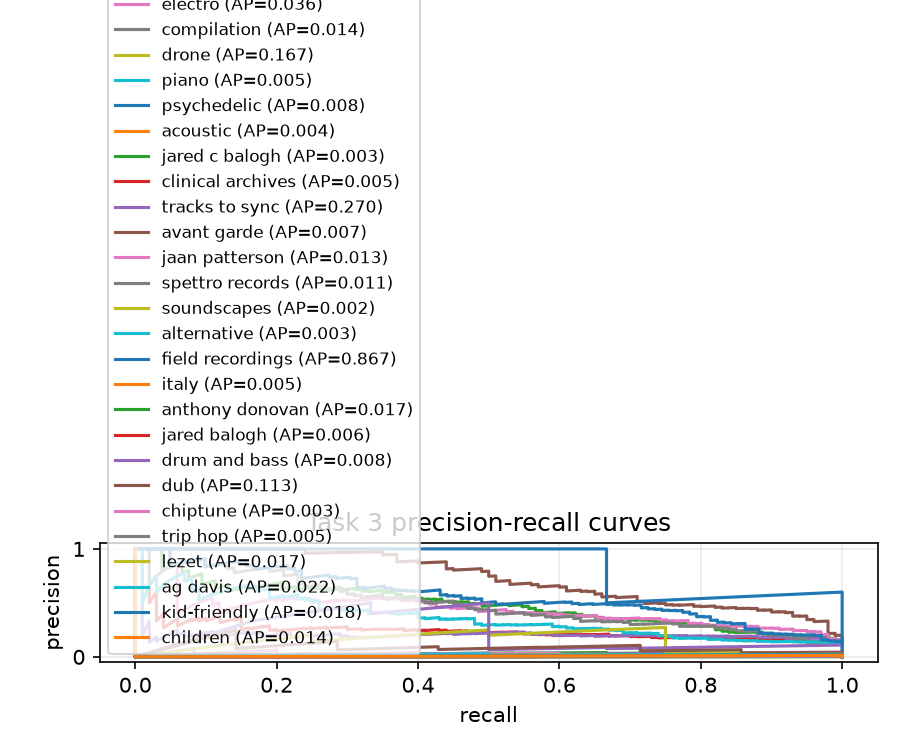
\includegraphics[width=\columnwidth]{task3_cross_attention_pr_curve.png}
\caption{Cross-attention test precision--recall curves across valid labels.}
\label{fig:task3-crossattn-pr}
\end{figure}

\section{Qualitative Analysis}
The cross-attention t-SNE visualization is shown in
Fig.~\ref{fig:task3-tsne}. It is used only as a qualitative diagnostic:
embedding neighborhoods may suggest label structure, but t-SNE does not
replace held-out evaluation. The remaining per-condition plot files remain
Additional per-condition diagnostic plots are retained with the experimental
artifacts; they are not reproduced here because they do not alter the
ablation conclusion.

Three case studies are available for the full cross-attention run. Each
case study contains the track identifier, text input, target labels,
predicted labels, and prediction scores. These examples are intended to
support inspection of graph/text agreement and failure modes. In particular,
the low macro-F1 of all multimodal conditions motivates checking rare-label
misses rather than presenting only successful examples.

\begin{figure}[!ht]
\centering
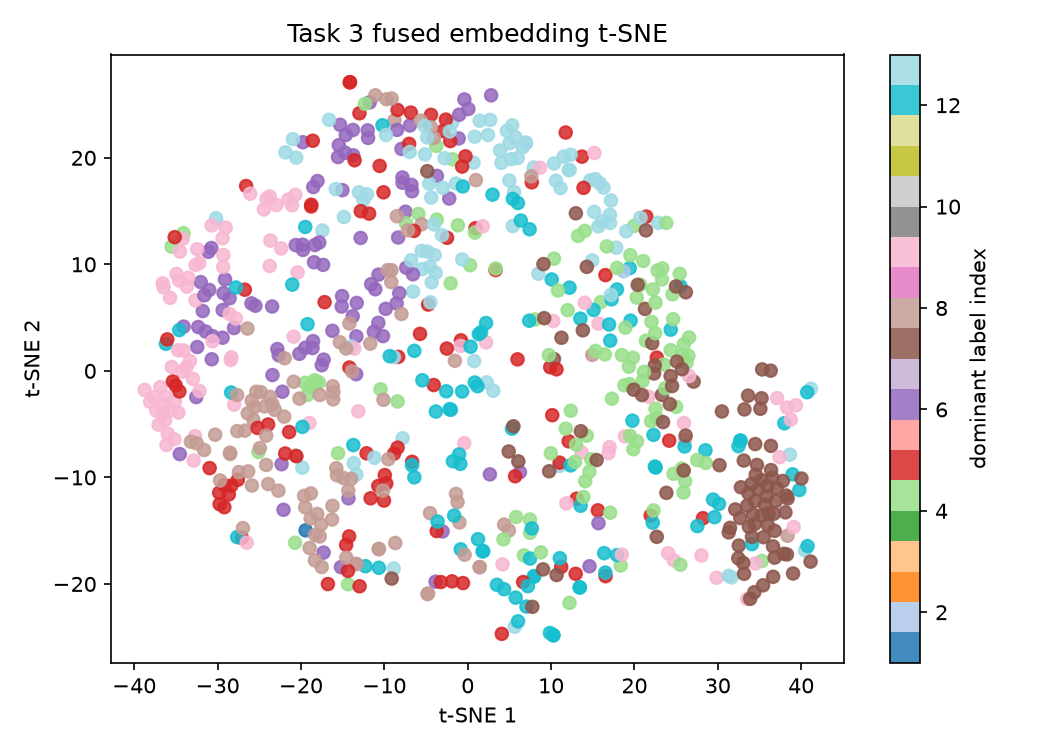
\includegraphics[width=\columnwidth]{task3_cross_attention_fused_tsne.png}
\caption{t-SNE projection of cross-attention fused test embeddings, shown
as a qualitative diagnostic rather than a performance metric.}
\label{fig:task3-tsne}
\end{figure}

\section{Discussion}
The results provide three practical conclusions. First, the text pipeline is
functional, but the caption-proxy construction makes its near-perfect score
an upper-bound-like diagnostic rather than a comparable benchmark. Second,
the rich segment graph is competitive with a simple audio CNN but does not
outperform it on the current FMA-small run; graph topology or the similarity
threshold may require further tuning. Third, the multimodal ablation confirms
that audio structure is the dominant signal for this label setup. Text
fusion improves micro-level decisions over BERT-only, yet does not improve
macro-F1 over GNN-only, suggesting label imbalance, limited usable text, or
optimization difficulty.

\section{Limitations and Future Work}
The present study does not include emotion regression or paired
graph--caption retrieval. Audio genre classification, caption-proxy
classification, and multimodal tag prediction use different supervision and
should not be compared directly. Exact full-data inventory counts are also
not available in the committed artifacts.

Several limitations remain. The caption-proxy target is a
caption-derived proxy, FMA metadata text is sparse and heterogeneous, and
the selected labels are imbalanced. The 0.5 threshold is global rather
than label-calibrated. The graph contains rich handcrafted statistics, but
the current study does not isolate each feature family or compare multiple
similarity thresholds. Finally, the reported runs use one seed; repeated-seed
confidence intervals are needed before claiming robust ranking differences.

\subsection{Future-work roadmap}
The next experiments follow directly from the preserved findings:
\begin{enumerate}
\item add per-label validation threshold tuning, calibrated probabilities,
and repeated seeds with confidence intervals;
\item compare class-balanced, focal, and asymmetric multi-label losses and
report rare-label versus frequent-label performance;
\item sweep graph similarity thresholds, adjacency variants, pooling
strategies, and feature ablations;
\item improve text coverage while maintaining strict exclusion of genre/tag
targets and artist identity shortcuts;
\item add the optional DEAM emotion head as a genuinely multi-task objective;
\item implement paired graph--caption contrastive learning and report
Caption-to-Audio and Audio-to-Caption Recall@1/5/10;
\item expand qualitative analysis with graph paths, attention maps, and
failure cases from all four ablations; and
\item package exact dataset counts, vocabulary frequencies, split summaries,
and preprocessing logs as supplementary reproducibility tables.
\end{enumerate}

\section{Artifact Map for Reproduction}
The analysis is backed by structured artifacts rather than screenshots alone.
The text baseline uses the metrics, test-metrics, predictions, and F1-curve
files under \texttt{results/task1}. The genre models use both model metric
files, predictions, learning curves, confusion matrices, and
\texttt{task2\_model\_comparison.json}. The multimodal analysis uses one
metrics, prediction,
case-study, learning-curve, PR-curve, and t-SNE bundle per condition, plus
\texttt{task3\_ablation\_comparison.json} and
\texttt{task3\_ablation\_analysis.txt}. Source modules under \texttt{src/}
define the preprocessing and training contracts, while \texttt{README.md}
contains the sequential commands needed to regenerate the pipeline.

\section{Conclusion}
We implemented a reproducible BERT, GraphSAGE, and graph--text fusion
pipeline for music context understanding. On the current real-run outputs,
the mel-CNN is the strongest genre classifier, while graph representations
are the strongest source of macro-level multi-label signal. The
ablation results support multimodal fusion as a useful direction, but also
make clear that future gains require stronger supervision and improved
generalization to rare labels.

\bibliographystyle{IEEEtran}
\bibliography{references}
\end{document}
